\chapter{Ratios, Functions, and Beyond}

\section{Ratios and Proportional Relationships}
As a topic in school mathematics, ratios and proportions are often isolated entities with their own special vocabulary, habits, and procedures.  When studying ratios and proportional situations, students often learn, ``Set up a proportion and cross multiply.''   But what is a proportion?  When does cross multiplication work?  Why does it work?  

For the problems in this section, try to take a more general approach:  ``Write an equation and solve.''  More precisely, ``Write an equation relating the quantities, and solve the equation for the desired quantity (usually an unknown).''  These are skills that serve students well throughout school mathematics and beyond.  

As you work through the problems and activities for this section, you will find it useful to make use of reasoning tools such as the following:  
\begin{itemize}
\item Equivalent fractions
\item Equivalent ratios
\item Ratio tables
\item Unit rates
\item Double number lines
\item Graphs
\end{itemize}

During the process, be on the lookout for a wide variety of strategies, including part:part comparisons, part:whole comparisons, common denominators, and common numerators.  And note how the problems simultaneously build on understandings of fractions and pave the way for functions.  

\subsection{Ratios}
Fractions, ratios, and rates are three connected ideas with differing histories and differing usage: 
\begin{itemize} 
\item \emph{Fractions} are numbers, often used to express results of sharing, cutting, or measuring.  
\item \emph{Ratios} have historically been used to compare quantities of the same kind, such as two lengths or two volumes.  Ratios are often expressed as pairs of counting numbers, without units, e.g., $3:2$.  
\item \emph{Rates} are typically used to compare different quantities (e.g., meters and seconds).  Rates are often expressed as quotients with units (e.g., 1.5 m/sec).  
\end{itemize} 

In high school and beyond, these rough historical distinctions become blurred, and the uses of these terms are varied, sometimes conflicting, and often muddled.  Thus, we will not attempt to write precise definitions that distinguish these terms from one another.  Instead, we aim toward the end-goal that students see all of these as quotients that provide differing perspectives on closely related ideas.  

To this end, we invest our energy in solving problems.  We will see that it is sometimes useful to attend only to the numbers in a situation, so that we can notice that two apparently different problems are abstractly the same if we ``decontextualize'' the problem by removing the units.  At other times, we will see the importance of using the units to interpret answers in context.  This interplay is the essence of modeling.

\fixnote{It would help to have some discussion of ``unit'' as 1, unit in measurement, and unit in a unit rate.}

\begin{teachingnote}
You will find insightful discussion and pictures in the draft 6-7 Progression on Ratios and Proportional Relationships, available at 

\url{http://math.arizona.edu/~ime/progressions/}
\end{teachingnote}

\subsection{Proportional Relationships}
For situations that involve two varying quantities, perhaps the most fundamental are those in which the quantities are proportional to one another.  
\begin{definition}
Quantities $x$ and $y$ are in a \emph{proportional relationship} if there is a constant $k$ such that $y=kx$.  
\end{definition}
When solving problems, a critical skill is the ability to distinguish propotional situations from situations in which quantities are not proportional.  
\begin{question}
Give a table of data for two quantities that are in a proportional relationship.  
\end{question}
\QM

\begin{question}
Give a table of data for two quantities that are \textbf{not} in a proportional relationship.  
\end{question}
\QM


\begin{activitynote}
Activities \ref{A:ratioLaunch}, \ref{A:ratios},  and \ref{A:ratioOddities} complement this section well. 
%% Ratio Launch
%% Poor Old Horatio
%% Ratio Oddities
%% Problem Solved
As a conclusion, we suggest doing Activity \ref{A:dreadedStoryProblem}.
\end{activitynote}

\newpage
\begin{problems}

\fixnote{Need easy problems, strip diagrams, double number lines.  See Beckmann.} 

\begin{enumerate}
\item A baseball coach once asked me the following question: If a
  pitcher can throw a 90 mph pitch during a game, but can only
  sustain a 60 mph pitch during practice, how close should the pitcher
  stand during practice to ensure that the amount of time it takes the
  ball to reach home plate is the same in practice as it is in the
  game? Explain your reasoning.

\item Three brothers and a sister won the lottery together and plan to
  share it equally. If the brothers alone had shared the money, then
  they would have increased the amount they each received by \$20. How
  much was won in the lottery? Explain your reasoning.

\item Chris is working on his Fiat. His car's cooling system holds 6
  quarts of coolant, and should be filled with a 50/50 mix of antifreeze 
and water. Chris noticed that the car was 1 quart low with the correct 50/50 mix.  
But then he added a 25/75 mix, 25 parts antifreeze, and 75 parts water.  How
  much coolant does he have to remove from the cooling system to then
  add 100 percent antifreeze to restore his desired 50/50 mix? Explain
  your reasoning.

\item If a hen and a half lays an egg and a half in a day and a half, 
how many eggs will 6 hens lay in 4 days?  How many days will it take for 
8 hens to lay 16 eggs?  How many hens would it take to lay 12 eggs in 
three days?  How many hens would it take to lay a dozen eggs per week?  
In each case, explain your reasoning.  

\item Fred and Frank are two fitness fanatics on a run from $A$ to
  $B$. Fred runs half the way and walks the other half. Frank runs for
  half the time and walks for the other half. They both run at the
  same speed and they both walk at the same speed. Who finishes first?
\begin{enumerate}
\item Before any computations are done, guess the
  solution to this problem and record your guess.  
\item Try to get a feel for this problem by choosing numbers for the
  unknowns and doing some calculations. What do these calculations say
  about your initial guess?
\item Use algebra to solve the problem.  What does your solution say 
about your initial guess?  
\end{enumerate}

\item Andy and Sandy run a race of a certain distance. When Sandy finishes, 
she is $1/10$ of the distance ahead of Andy, who then finishes the race. 
After some discussion, Andy and Sandy decide to race the distance again, but this time Sandy
  will start $1/10$ of the distance behind Andy (at the starting line) to ``even-up'' the
  competition. Who wins this time?  Explain your reasoning.  
\begin{enumerate}
\item Before any computations are done, guess the
  solution to this problem and record your guess.  
\item Try to get a feel for this problem by choosing numbers for the
  unknowns and doing some calculations. What do these calculations say
  about your initial guess?
\item Use algebra to solve the problem.  What does your solution say 
about your initial guess?  
\end{enumerate}

\item You have two beakers, one that contains water and another that
  contains an equal amount of oil. A certain amount of water is
  transferred to the oil and thoroughly mixed. Immediately, the same
  amount of the mixture is transferred back to the water. Is there now
  more water in the oil or is there more oil in the water?
\begin{enumerate}
\item Before any computations are done, guess the
  solution to this problem and record your guess.
\item Try to get a feel for this problem by choosing numbers for the
  unknowns and doing some calculations. What do these calculations say
  about your initial guess?
\item Use algebra to solve the problem.  What does your solution say 
about your initial guess?  
\end{enumerate}

\item While on a backpacking trip Lisa hiked five hours, first along a
  level path, then up a hill, then turned around and hiked back to her
  base camp along the same route. She walks $4$ miles per hour on a
  level trail, $3$ uphill, and $6$ downhill. Find the total distance
  traveled. Explain your reasoning.
\item Monica, Tessa, and Jim are grading papers. If it would take
  Monica $2$ hours to grade them all by herself, Tessa $3$ hours to
  grade them all by herself, and Jim $4$ hours to grade them all by
  himself how long would it take them to grade the exams if they all
  work together? Explain your reasoning.
\item Say quickly, friend, in what portion of a day will four
  fountains, being let loose together, fill a container which would
  be filled by the individual fountains in one day, half a day, a
  third of a day, and a sixth of a day respectively? Explain your
  reasoning---note this is an old problem from the Indian text
  \textit{Lilavati} written in the 1200s.
\item Three drops of \textit{Monica's XXX Hot Sauce} were mixed with
  five cups of chili mix to make a spicy treat---the hot sauce is much
  hotter than the chili. Later, two drops of \textit{Monica's XXX Hot
    Sauce} were mixed with three cups of chili. Which mixture is
  hotter? 

Josh made the following observation:  ``If two different recipes are added 
together, the result will be a chili with hotness between the two.''  Explain
why this makes sense.  

To compare the given recipes, Josh suggested using this reasoning backwards, 
as follows:  
 
\begin{itemize}
\item Remove the second (recipe) from the first, that is: Start with 3
  drops of hot sauce and 5 cups of chili, and remove 2 drops and 3
  cups. So we are now comparing
\[
\text{1 drop and 2 cups}\qquad\text{with}\qquad\text{2 drops and 3 cups.}
\]
\item Now remove the first from the second, that is: Start with 2
  drops and 3 cups, and remove 1 drop and 2 cups. So we are now
  comparing
\[
\text{1 drop and 2 cups}\qquad\text{with}\qquad\text{1 drop and 1
  cup.}
\]
\end{itemize}
Now you can see that the second is more concentrated (and hence
hotter!) than the first. Is this correct? Will this strategy
always/ever work? Explain your reasoning.
\end{enumerate}
\end{problems}

\section{Sequences and Functions}
\paragraph{Sequences.}  Because "Sequences and Series" is a common topic in calculus and precalculus courses, the concept of sequence is often considered an advanced topic in high schools, but the idea of a sequence is much more elementary.  In fact, many patterns explored in grades K-8 can be considered sequences.  For example, the sequence $4, 7, 10, 13, 16, \dots$ might be described as a ``plus 3 pattern'' because terms are computed by adding 3 to the previous term.  
\begin{activitynote}
Activities \ref{A:walk} through \ref{A:ExponentRules} are intended for this section.  
%%  Walk the Line  \ref{A:walk} 
%%  Constant Amount Change  \ref{A:ConstantAmount}
%%  Constant Percentage (Ratio) Change  \ref{A:ConstantRatio}
%%  Rules of Exponents  \ref{A:ExponentRules}
%%  Garden Variety \ref{A:gardenVariety}
\end{activitynote}
\begin{definition}
A \textbf{sequence}\index{sequence} is an ordered set of numbers or other objects.  The numbers or objects are called the \textbf{terms} of the sequence.  
\end{definition}

\paragraph{Functions.}  In the Common Core State Standards, students begin formal study of functions in grade 8.\standard{8.F.1}  
In high school, the approach to functions becomes more formal, through the use of function notation and with explicit attention to the concepts of domain and range.\standardhs{F-IF.1}   

\begin{definition}
A \textbf{function}\index{function} is a rule in which each input value determines a corresponding output value.  The \textbf{domain}\index{domain} of a function is the set of input values.  The \textbf{range}\index{range} of the function is the set of output values.
\end{definition}

\paragraph{Sequences Are Functions.} As students begin formal study of functions, it makes sense to use their patterning experience as a foundation for understanding functions.\standardhs{F-IF.3}  To show how the sequence above can be considered a function, we need an \textit{index}, which indicates which term of the sequence we are talking about, and which serves as an input value to the function.  After deciding that the 4 corresponds to an index value of 1, we can make a table showing 
the correspondence.\marginfigure{\footnotesize\sffamily
      \begin{tabular}{c||c|c|c|c|c|c}
        $n$ & 1 & 2 & 3 & 4 & 5 & \dots \\
\hline
        $f(n)$ & 4 & 7 & 10 & 13 & 16 & \dots
      \end{tabular}
\normalfont}

%%  \margincomment{We recommend using subscript notation only in advanced high school courses.} 

Although sequences are sometimes notated with subscripts, function notation can help students remember that sequences are functions.  For example, the sequence can be described recursively by the rule $f(1) = 4$, $f(n+1) = f(n) + 3$ for $n \geq 2$.  Notice that the recursive definition requires both a starting value and a rule for computing subsequent terms.   
The sequence can also be described with the closed (or explicit) formula  $f(n) = 3n + 1$, for integers $n \geq 1$.  Notice that the domain (i.e., integers $n\geq 1$) is included as part of the description.  When a function is given without an explicit domain, the assumption is that the domain is all values for which the expression is valid.  Thus, the function $g(x) = 3x + 1$ appears to be essentially the same as the function $f$ because the formula is the same and because $f(n) = g(n)$ for all positive integers.  To see that the functions are different, observe that $g(2.5) = 8.5$, but $f(2.5)$ is undefined.  

A common habit in school mathematics is creating a table of $(x,y)$ pairs, plotting those pairs (as dots), and then ``connecting the dots.''  The above discussion demonstrates that this habit is sometimes not appropriate: A graph\marginfigure{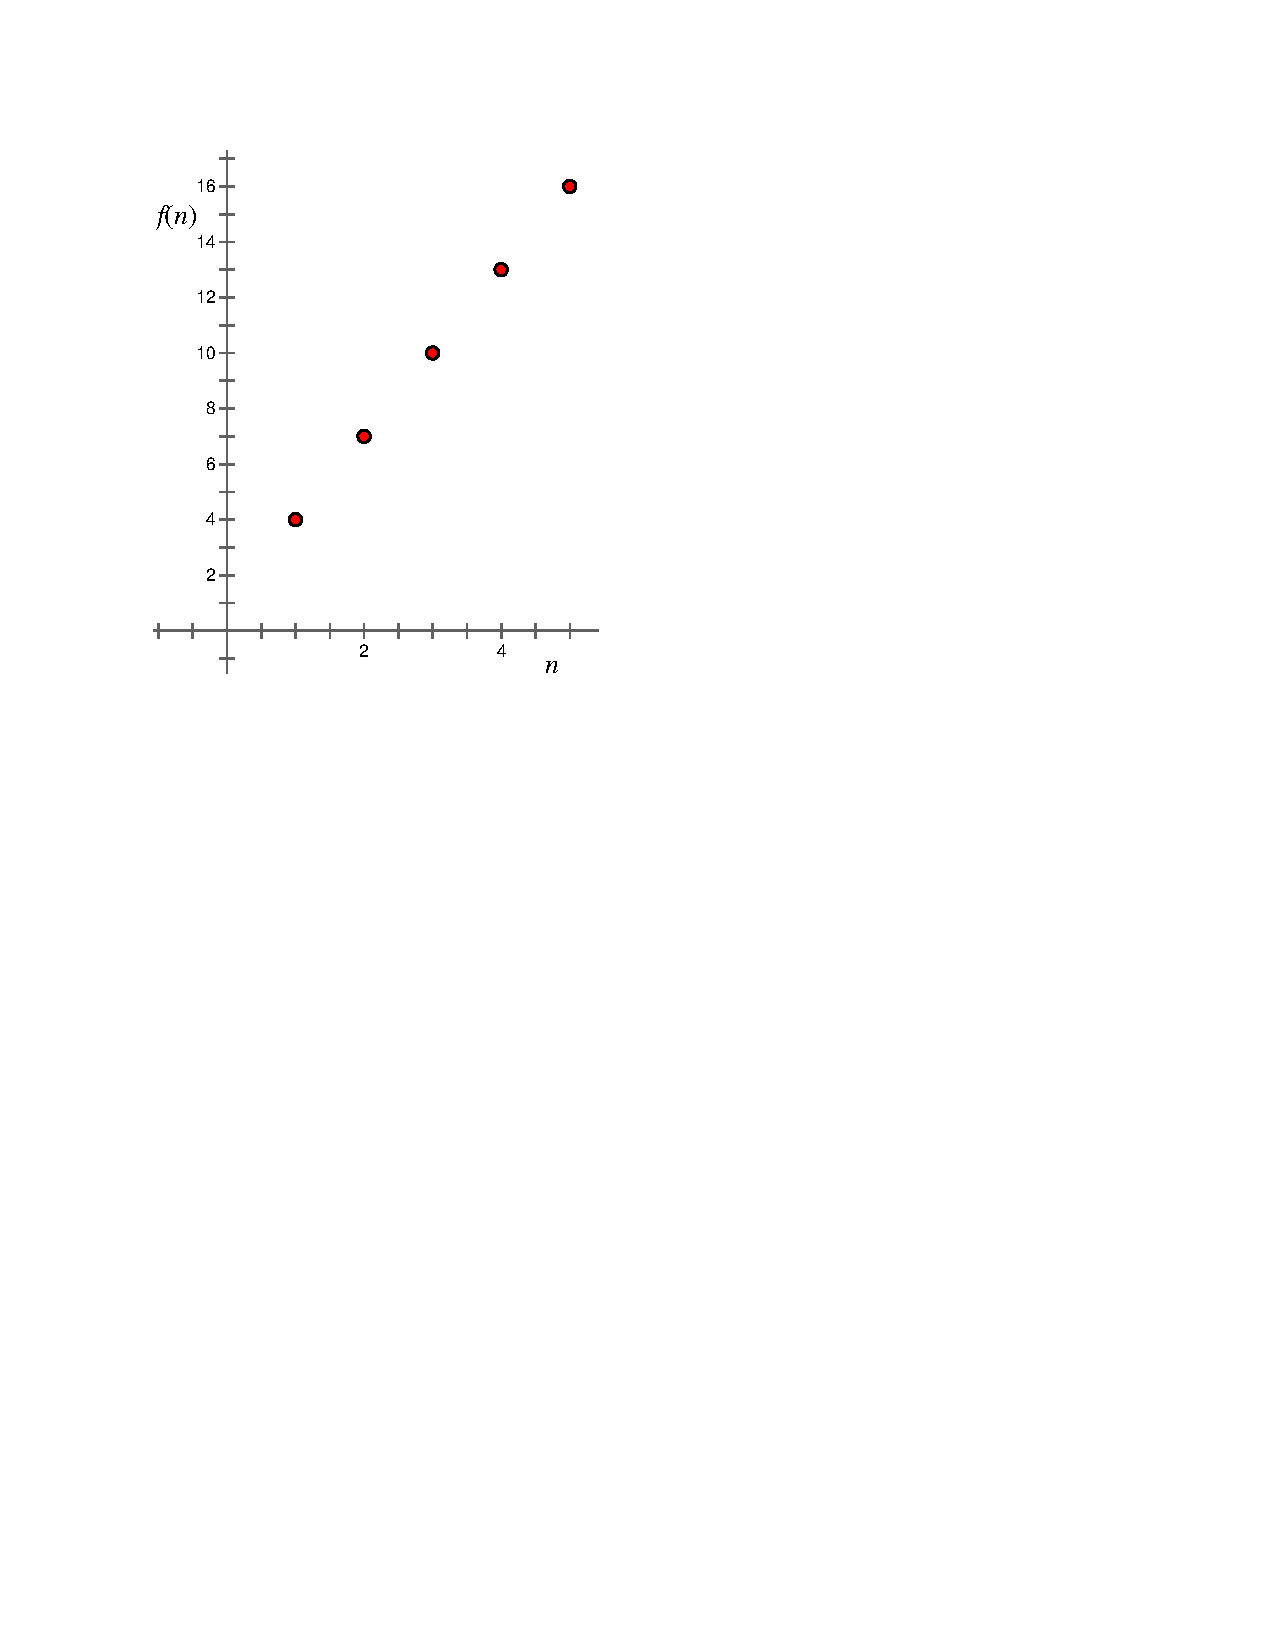
\includegraphics[width=2in]{../graphics/Graph-F2.pdf}} 
of the sequence consists of discrete dots, because the specification does not indicate what happens ``between the dots.''  Connecting the dots requires the assumption that domain values between the dots make sense in some way.  


\begin{question}
In your own words, what does it mean to say that sequences are functions?
\end{question}
\QM

\begin{question}
Given that $g(1) = 3$ and $g(n+1) = g(n) +4$ for integers $n>1$, find $g(6)$.  
Find a closed formula for $g(n)$.  
\end{question}
\QM

\begin{question}
Given that $f(1) = f(2) = 1$, and $f(n+1) = f(n)+f(n-1)$ for integers $n>2$, find $f(6)$.  
\end{question}
\QM

\paragraph{Arithmetic and Geometric Sequences.}Two types of sequences are especially important.\standardhs{F-BF.2}  
\begin{definition}
An \textbf{arithmetic sequence} any sequence that has a constant difference between consecutive terms.  A \textbf{geometric sequence} has a constant ratio between consecutive terms.  Some sequences, of course, are neither arithmetic nor geometric.
\end{definition}
\begin{question}
For each of the following sequences, decide whether it is arithmetic, geometric, or neither, and explain your reasoning:
\begin{itemize}  
\item $1, 4, 9, 16, 25, \dots$
\item $4, 8, 16, 32, \dots$
\item $2, 4, 6, 8, 2, 4, 6, 8, \dots$
\item $-2, 5, 12, 19, \dots$
\end{itemize}
Can you write both recursive and explicit formulas for each of these sequences?  
\end{question}
\QM

Beginning in about grade 8, much of school mathematics is devoted to the study of linear, quadratic, and exponential functions.\standardhs{F-LE.2}  Here we provide only definitions and key questions about these types of functions.  

\begin{itemize}
\item A linear function is of the form $f(x) = ax + b$, where $a$ and $b$ are real numbers and $a\ne 0$.  What do $a$ and $b$ tell you about the linear function?  
\item A quadratic function is of the form $f(x) = ax^2 + bx + c$, where $a$,  $b$, and $c$ are real numbers and $a\ne 0$.  What do $a$, $b$, and $c$ tell you about the function?   
\item An exponential function is of the form $f(x)=ab^x$, where $a$ and $b$ are real numbers, $a\ne 0$, and $b>0$.  What do $a$ and $b$ tell you about the function? 
\end{itemize}

\begin{question}
Why do these definitions require that $a \ne 0$?  
\end{question}
\QM

\begin{question}
Why does the definition of exponential function require that $b > 0$?  What happens if $b=0$?  What happens if $b<0$?
\end{question}
\QM

How can you identify these types of functions in tables, graphs, symbols, and contexts?\standardhs{F-IF.4} \standardhs{F-IF.7}  
For example, how can you recognize the slope in the graph of a linear function?  What about in a table, in a symbolic expression, or in a context?  

\begin{question}
An arithmetic sequence is what kind of function?  Explain. 
\end{question}
\QM

\begin{question}
A geometric sequence is what kind of function?  Explain.  
\end{question}
\QM

\begin{question}
Sometimes quadratic functions are written in the form $f(x) = a(x-h)^2+k$, where $a$, $h$, and $k$ are real numbers and $a\ne 0$.  What do $a$, $k$, and $h$ tell you about the function?  What are the advantages and disadvantages of this form of a quadratic, as compared to the alternative form given above?  
\end{question}
\QM

\paragraph{Concluding Remarks.}  When studying arithmetic and geometric sequences, it is tempting to encapsulate common results into compact formulas.  But formulas are easily confused with one another and otherwise misremembered.  Furthermore, general formulas often obscure the ideas.  

\begin{question}
Find the missing terms in the following arithmetic sequence:  
$$\rule[-2pt]{25pt}{.5pt}, \rule[-2pt]{25pt}{.5pt},  2,  \rule[-2pt]{25pt}{.5pt}, \rule[-2pt]{25pt}{.5pt}, 6, \dots$$
Explain your reasoning.  
\end{question}

\begin{question}
Find exact values (not decimal approximations) for the missing terms in the following geometric sequence:  
$$\rule[-2pt]{25pt}{.5pt}, \rule[-2pt]{25pt}{.5pt},  2,  \rule[-2pt]{25pt}{.5pt},  \rule[-2pt]{25pt}{.5pt}, \rule[-2pt]{25pt}{.5pt}, 6, \dots$$
Explain your reasoning.  And describe how this problem and the rules of exponents might be used to explain the connection between radicals and exponents.  
\end{question}

\begin{question}
What key ideas behind arithmetic and geometric sequences did you use in the previous two problems? 
\end{question}

\begin{center}
\textbf{With the ideas, you can reconstruct the formulas you need.  And without the ideas, formulas are empty.}  
\end{center}

\newpage
\begin{problems}
\begin{enumerate}

\item A park consists of a row of circular gardens.  ``Garden \#0'' has radius 3 feet, and each successive garden after that has a radius 2 feet greater than the previous garden.  
\begin{enumerate}
\item Using tables as a guide, write both explicit and recursive representations that will allow us to predict the area of the $n^\mathrm{th}$ garden.
\item Make a graph that shows the areas of the gardens in the park.  Which variable do you plot on the horizontal axis?  Explain.  
\item Does it make sense to connect the dots on your graph?  Explain your reasoning.  
\item Using your table, compute the area differences between the successive gardens.  What do you notice?  Why does this happen?
\end{enumerate}
\item An oil spill starts out as a circle with radius 3 feet and is expanding outward in all directions at a rate of 2 feet per minute. 
\begin{enumerate}
\item Use tables, graphs, and formulas to describe the area of the oil region $x$ minutes after the spill.  
\item How is this question fundamentally different than that of the gardens?  
\item Dumb Question:  At any one time, how many different areas are possible for the oil region?
\end{enumerate}


%\begin{prob}
%\textbf{Domain in context.}  Recall that the domain of a function is the set of input values that make sense in the problem.  Consider the following problem contexts:  
%\begin{itemize}
%\item The County Fair costs \$7 for admission and \$4 for each ride.  
%\item A taxi company charges \$11 for the first mile (or fraction thereof) and \$4 for each additional mile (or fraction thereof).  
%\item The Halloween parade, moving at a constant speed, was at mile marker 7 at noon, and at mile marker 11 at 1 pm.  
%\end{itemize}
%Blair used the letters $f$, $g$, and $h$ to describe functions for these three contexts, respectively, and noticed that 
%$f(3)=g(3)=h(3)$.  When she found a single formula that seemed to work for all three contexts, she thought that the three functions were equal.  But when she drew careful graphs of the functions, she was able to see that although the functions agree on many input values, they also disagree on many others.  
%
%Recreate Blair's work.  For each function, describe the meanings of the input and output values.  Indicate the domain of each function, and extend the domain, where reasonable, to include 0, fractions that are not counting numbers, and negative values.  Be sure that both the input and output values fit the context.  Draw a graph for each function, and describe how the graphs show the ways that the functions are both the same and different.  
%\end{prob}
%
%\begin{prob}
%The table below represents population growth for a hypothetical rabbit population.  
%
%\begin{center}
%\begin{tabular}{|l|c|c|c|c|c|}
%\hline
%Time (yrs) & 0 & 1 & 2 & 3 & 4 \\ \hline
%Population & 100 & 180 & 325 & 583 & 1,050\\  \hline
%\end{tabular}
%\end{center}
%
%\begin{enumerate}
%\item Assuming the growth pattern continues, write an equation for the rabbit population $p$ for any year $n$ after the rabbits are first counted.  Explain what the numbers in your equation represent. 
%\item Use your equation and this context to explain the meaning of an exponent of $-3$.  
%\item Based on common knowledge about rabbit populations, what can you say about the domain of your model?  In other words, what are the $n$-values for which the model is potentially reasonable?  
%\item In order to explore the accuracy of your exponential model for this rabbit population, write an equation for the rabbit population $p$ for any month $m$ after the rabbits are first counted.  Show how you know that your new equation describes the same population of rabbits.  
%\end{enumerate}
%Note:  This problem is based upon Problem 3.1 from \emph{Growing, Growing, Growing}, an eighth grade unit from CMP2, the second edition units of the Connected Mathematics Program. 
%\end{prob}
%
%
%\begin{prob}
%Suppose we want to fill in the blanks in the following geometric sequence: 
%\[ 
%\rule[-2pt]{35pt}{.5pt}, \rule[-2pt]{35pt}{.5pt}, \quad 2, \rule[-2pt]{35pt}{.5pt}, \rule[-2pt]{35pt}{.5pt}, \rule[-2pt]{35pt}{.5pt}, 
%\quad 6, \rule[-2pt]{35pt}{.5pt}, \dots
%\]
%\begin{enumerate}
%\item Why would it be incorrect to place 3, 4, and 5 in these blanks between 2 and 6? 
%\item Find exact values (not decimal approximations) for the missing values. Explain your reasoning. 
%\item Amanda used radicals to solve this problem, but Justin used exponents. Explain how both approaches can be correct. 
%\item Suppose $b$ is $n$ terms after $a$ in a geometric sequence. Find the $k^{th}$ term after $a$. Explain your reasoning. 
%\end{enumerate}
%\end{prob}
%
%%4. Geometric Sequences.  A sequence of numbers is called a geometric sequence if there is a constant ratio between consecutive terms.  For example, 2, 10, 50, 250, … is a geometric sequence with a starting term of 2 and a constant ratio of 5.  
%% 7.	Fill in the missing terms in the following geometric sequences: 
%% 
%% a.	5, ____, 15, ____, _____, …
%% b.	4, ____, ____, 20, ____, ____, …
%% c.	____, ____, ____, ____, ____, ____, ____, 4, ____, 8, ____, ____, …
%

  
%\begin{prob}
%Another way to reason about the meanings of zero and negative exponents is to use contexts involving exponential growth.  Suppose a virulent species of algae is overtaking the surface of a pond.  When scientists first noticed the problem, the algae covered 9 square meters of the pond surface.  One day later, the algae covered 18 square meters.  
%\begin{enumerate}
%\item Assuming the algae cover doubles every day, what will the algae coverage be on day 5?
%\item Write an expression that gives the algae coverage on any day. 
%\item On what day will the algae cover the whole pond, which measures about 10,000 square meters?  What does your answer say about your expression in part b?  
%\item  Use your expression and the context to interpret 0 and negative integer exponents.  
%\end{enumerate}
%\end{prob}
%
%\begin{prob}
%To make sense of an exponent of 1/2, Drew suggested that if the algae covered 9 square meters at noon on day 0 and 18 square meters at noon on day 1, then at 1/2 day, there would be 13.5 square meters of algae, which is 1.5 times as much.  Kelsey pointed out that if there is 1.5 times as much algae after 1/2  day, then there would be $1.5\cdot1.5 = 2.25$ times as much algae after a full day, which does not fit the context.  
%\begin{enumerate}
%\item Assuming that the algae has a constant growth factor, how much algae should there be at  1/2  day?  
%\item How does this help determine what an exponent of 1/2 should mean?  Explain.
%\item How much algae will there be after 1/3 of a day?  Express your answer using exponents, and approximate it as a decimal.
%\end{enumerate}
%\end{prob}


\end{enumerate}
\fixnote{Need more problems.  Doubling time?  Half life?  Use the ones from HW 8, in comments above.}



\end{problems}

\newpage

\section{Series}  
\begin{definition}
A \textbf{series} is a sum of consecutive terms from a sequence.  A series with terms that form an arithmetic sequence is called an \textbf{arithmetic series}.  
\end{definition}

\begin{activitynote}
Activities \ref{A:arithmeticSeries} and \ref{A:geometicSeries} are intended for this section.  
\end{activitynote}

\begin{question}
Find the sum:  $1 + 3 + 5 + \dots + 4999.$  (First explain how you know this is an arithmetic series.)
\end{question}
\QM

In mathematics teaching and learning, it is useful to distinguish problems from  excercises. \emph{Problems} require that you formulate a solution strategy, whereas \emph{exercises} are about using a procedure that you have been taught.\margincomment{Problem solving is an essential part of mathematics.}  Whether a question is a problem or an exercise depends upon the learner.  
\begin{question}
Is the previous question a problem or an exercise for you?  
\end{question}

When analyzing any series, it is often useful to consider the \emph{sequence of partial sums}.  For example, in response to the above question, the sequence of partial sums is as follows:  $$1, \qquad 1 + 3, \qquad 1+ 3+5, \qquad 1+3+5+7, \qquad \dots$$

Sometimes you can see a pattern in the sequence of partial sums.  Making a conjecture about a pattern is a type of inductive reasoning.  Once you notice a pattern, an important next step is showing, deductively, that the pattern \emph{must} continue.  

For arithmetic series, here are some approaches that can lead to general deductive arguments for the sum: 

\begin{itemize}
\item Consider pairing the first term with the last term, the second term with the second-to-last term, and so on.  What do you notice about the sum of each of these pairs?  And how many such pairs are in the whole series?  
\item Consider the average of each of the same pairs.  How might those averages help determine the sum of the whole series?  
\item Consider writing the series backward immediately below a forward version, line up the terms, and then add vertically.  
\end{itemize}

\begin{question}
Use one of these approaches to show that the sum is what it is.  Can you use a picture to illustrate your reasoning?    
\end{question}
\QM

\begin{question}
When you consider the sequence of partial sums of an arithmetic series, what kind of function(s) can you get?  Explain.  
\end{question} 
\QM

\begin{definition}
A series with terms that form a geometric sequence is called a \textbf{geometric series}.  
\end{definition}

\begin{question}
Find the sum:  $\frac{2}{3}+\frac{2}{9}+\dots+\frac{2}{3^{10}}$.  (First explain how you know the series is geometric.)
\end{question}
\QM

For the question above, it is not hard to see a pattern in the sequence of partial sums.  In fact, it is reasonable to believe that the pattern holds for any (finite) partial sum of the infinite geometric series $\frac{2}{3}+\frac{2}{9}+\dots$.  But to show that the pattern always holds, we need a general argument.  

For geometric series, the techniques for arithmetic series do not carry over.  Instead, observe that if you multiply the series by the common ratio, the resulting series has most of the same terms as the original series.  Thus, the difference between the two series (i.e., subtract the two) is a short expression that is not hard to work with.  

\begin{question}
Use these ideas to show that the sum is what it is.  Can you use a picture to illustrate this sum?    
\end{question}
\QM

\begin{question}
Convert $0.\overline{42}$ to a fraction.  What connections do you see with geometric series?  
\end{question}
\QM

\begin{question}
Explain briefly the key ideas behind finding the sum of an arithmetic series. Then do the same for geometric series.  
\end{question}
\QM


\newpage
\begin{problems}
\begin{enumerate}


\item Recall the story of Gertrude the Gumchewer, who has an addiction to Xtra Sugarloaded Gum.  Each day, she goes to her always stocked storage vault and grabs gum to chew.  At the beginning of her habit, she chewed three pieces and then, each day, she chews eight more pieces than she chewed the day before to satisfy her ever-increasing cravings. We want to find out how many pieces of gum did Gertrude chew over the course of the first 973 days of her habit?

\item Assume now that Gertrude, at the beginning of her habit, chewed $m$
pieces of gum and then, each day, she chews $n$ more pieces than she
chewed the day before to satisfy her ever-increasing cravings.  How many pieces will she chew over the course of the first $k$
  days of her habit? Explain your formula and how you know it will work for any $m$, $n$ and $k$.  

\item Find the sum:
\[
19 + 26 + 33 + \dots + 1720
\]
Give a story problem that is represented by this sum.

\item Now remember the story of Billy the bouncing ball.  He is dropped from a height of 13 feet and each bounce goes up 92\% of the bounce before it.  Assume that the first time Billy hits the ground is bounce \#1.  How far did Billy travel over the course of 38 bounces (up to when he hits the ground on his 38th bounce)?  

\item Assume now that Billy the Bouncing Ball is dropped from a height of
$h$ feet. After each bounce, Billy goes up a distance equal to $r$
times the distance of the previous bounce. (For example, $r=.92$ above.)
\begin{enumerate}
\item How high will Billy go after the $k$th bounce?
\item How much distance will Billy travel over the course of $k$
  bounces (not including the height he went up after the $k$th
  bounce)?
\item If $r<1$, what can you say about Billy's bounces? What if $r=1$?
  What if $r>1$?
\end{enumerate}

\item Joey starts out with \$456.  He plays one hand of poker each day with the same stakes of \$10.  Because he doesn't know anything about poker, he is on an extended losing streak.  Write explicit and recursive representations for the amount of money Joey has after $n$ days.  
      
\item Suppose Buzz Aldrin could fold a piece of paper in half as many times as he wanted---for rectangular paper of any size.  How many folds would Buzz need for the thickness of the paper to reach or exceed the distance from the earth to the moon?  How many folds would it take to reach or exceed halfway to the moon?

\item A ball is thrown up in the air from a 200 foot cliff with an initial velocity of 15 feet per second.  What is the height of the ball at any time $t$?  Write explicit and recursive representations of the relationship between the time after the ball is thrown and its height above the base of the cliff.

\item While waiting for Mark Pi to arrive to address the Mathematics Party, the members all shake hands with one another.  When Mark Pi walks in, he shakes hands with only the big-wigs of the Party.  A total of 6357 handshakes took place that day, and no one shook hands with the same person more than once.  How many members were there?  How many big-wigs were there?

\item If you deposit \$347 at the beginning of each year (starting on Jan. 1, 2014), into an account that compounds interest annually at a rate of 6.7\%, how much will be in the account on January 2, 2056?

\item You take out a \$100,000 loan on Jan. 1, 2014 to buy one Michigan ticket.  The loan shark charges 13\% annual interest.  You agree to pay back the loan through equal annual payments beginning on Jan. 1, 2015 and ending with the final payment on Jan. 1, 2028.  How much should each annual payment be? How much interest will you pay over the course of the payment plan?  If you hit the lottery on Dec. 31, 2020 and decide to pay off the rest of the loan the next day, how much will you owe?

\item 5 mg of a drug are administered to a patient at the start of a treatment regimen.  Each day at the same time, 3 more mg of the drug is administered.  Assuming that the drug still dissipates by 21\% each day, how much of the drug will be in the body immediately following the 3$4^\mathrm{th}$ 3 mg dose?

\item Find the fractional representation of the number $0.78\overline{4396}$.

\item A park consists of a row of circular gardens.  The ``Garden 0'' has radius 3 feet, and each successive garden after that has a radius 2 feet longer than the previous garden.  If there are 37 gardens, how much total area would the gardens comprise?

\item During their hour play time, the two oldest Brady kids (Greg and Marcia) went to the park to play with their walkie-talkies.  They used them for an hour.  The next day, the next-oldest kid came along.  Because there were only two walkie-talkies, they needed to share so that each possible pair got equal time.  The next day, the next-oldest also came along.  This continued until on the ninth day, all ten kids were there wanting to use the walkie-talkies.  How much time did Greg and Marcia spend with each other on the walkie-talkies over the course of the nine days?

\item Find the total number of gifts given in the song ``The 365 Days of Christmas''.

\end{enumerate}
\end{problems}

